\documentclass[spanish]{udpreport}
\usepackage[utf8]{inputenc}
\usepackage[spanish]{babel}
\usepackage{float}


% Podemos establecer el logo de alguna entidad o dejar el de la UDP (defecto)
%\setlogo{EITFI}

\title{Informe Laboratorio IV \\ Redes de Datos}
\author{Arturo Mantinetti \\ Manuel Tobar \\ Diego Vilches \\ Nicolas Henriquez}
\email{arturo.mantinetti@mail.udp.cl \\ manuel.tobar@mail.udp.cl
	\\ diego.vilches@mail.udp.cl \\ nicolas.henriquez@mail.udp.cl}
	
\profesor{Profesor \\ Jaime Álvarez}
\ayudante{Ayudante \\ Maximiliano Vega}


\date{12 de Mayo de 2016}

% Además podemos establecer la facultad y escuela
% los valores por defecto son los siguientes:
%\udpschool{Escuela de Informática y Telecomunicaciones}
%\udpfaculty{Facultad de Ingeniería}
%\udpuniversity{Universidad Diego Portales}

\begin{document}
\maketitle

\tableofcontents

\chapter{Introducción}

Este laboratorio consistió en armar una simulación de red en Packet Tracer con distintos equipos y configuraciones dentro de la red para comprender el funcionamiento del protocolo SPT y las VLAN.

\chapter{Software utilizado}
La aplicación que usaremos en esta ocasión para simular las distintas redes sera Packet Tracer. Este programa es propiedad de Cisco y nos permite experimentar con el comportamiento de la red y resolver preguntas de que ocurriría con la red si realizamos cierta configuración o conexión de dispositivos.

\chapter{Actividades}

\section{Actividad I}
La primera actividad consiste en analizar los problemas producidos cuando una topología de red presenta enlaces redundantes y se generan bucles. Luego se comparan los resultados al incorporar el protocolo STP(IEE 802.1d) a los equipos de la red y se analizarán las ventajas que este ofrece a la hora de enfrentarse a la redundancia de la red.
 %insertar pantallazo de la red
 %si es posible rellenar con los switch  coloquenlos donde dejé un parentesis, si no borren el parentesis
La red consiste en tres switches()  conectados entre si. Luego se envían paquetes desde el switch0 hasta el switch2 y posteriormente desde el switch2 hasta el switch1.
%responder preguntas aquí.

En esta actividad montamos 3 switch Cisco interconectados como se muestra en la siguiente imagen 
\begin{figure}[H]
	\caption{Topologia Actividad I}
	\centering
	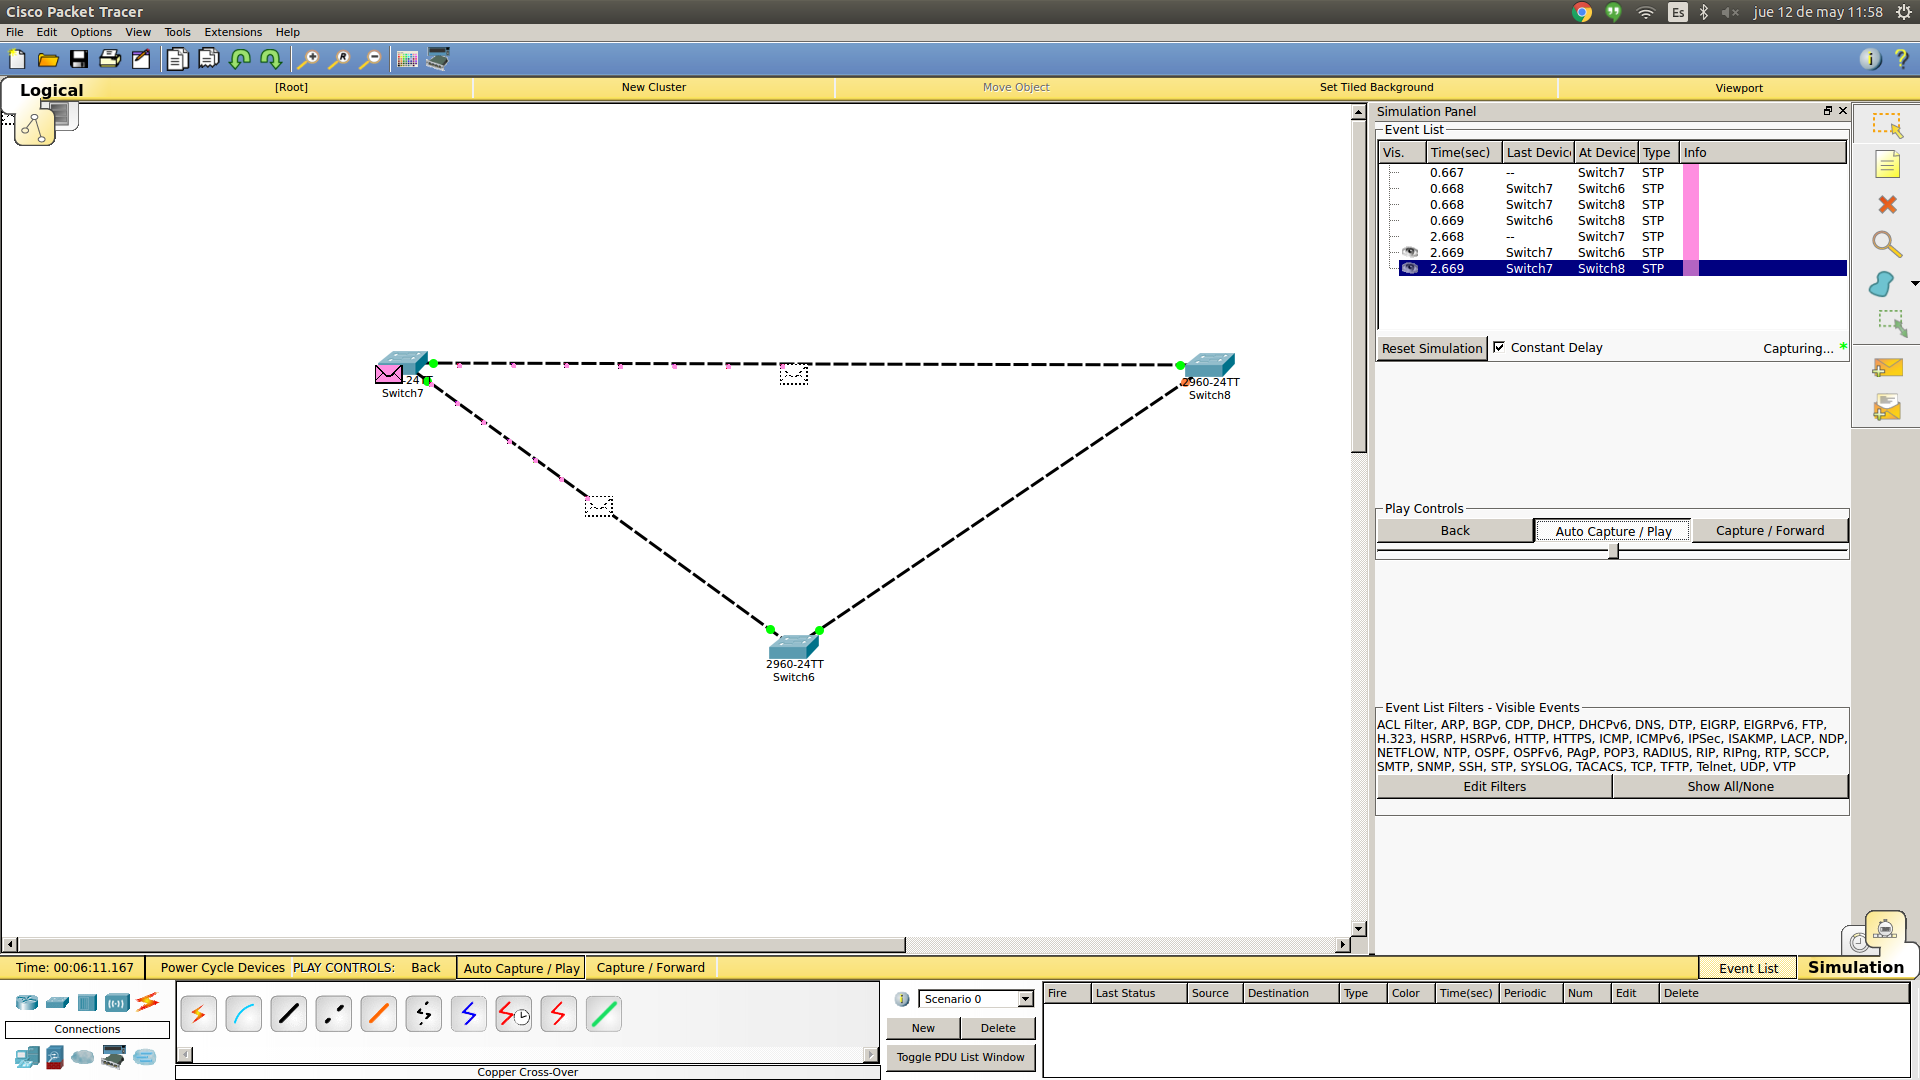
\includegraphics[scale=.25]{imagenes/A1.png}
	\label{fig:Figura 2.1}
	\linebreak
\end{figure}

\subsection{¿Qué camino realizara un paquete que para llegar desde el switch0 hasta el switch2?}
El paquete va directo desde el switch0 al switch2
\subsection{¿Qué camino realizara un paquete que para llegar desde el switch2 hasta el switch1?}
El paquete se dirige primero desde el switch2 al switch0 y luego se envia desde el switch0 al switch 1

\section{Actividad II}
Considerando la topología de la actividad I, se procede a configurar el switch1 como primario y el switch2 como secundario. Para lograr esto se deben ejecutar una serie de comandos en cada switch según como se vaya a configurar.
%poner en negrita o subtitulado o la wea que sea esto:
Para el switch primario:
\begin{flushleft}
	Switch>Enable \\
	Switch\#configure terminal \\
	Enter configuration commands, one per line. End with CNTL/ \\
	Switch(config)\#spanning-tree vlan 1 root primary \\
	Switch(config)\# \\
\end{flushleft}

Para el switch secundario:

\begin{flushleft}
	Switch>Enable \\
	Switch\#configure terminal\\
	Enter configuration commands, one per line. End with CNTL/\\
	Switch(config)\#spanning-tree vlan 1 root secondary\\
	Switch(config)\#\\
\end{flushleft}

 %responder las preguntas de la actividad 2

\subsection{¿Qué camino realizara un paquete que para llegar desde el switch2 hasta el switch0?}
El paquete se mueve directamente desde el switch2 al switch0
\subsection{¿Qué camino realizara un paquete que para llegar desde el switch1 hasta el switch0?}
El paquete se mueve directamente desde el switch1 al switch0


\section{Actividad III}
Para esta tercera actividad, se establecerá una prioridad para cada uno de los tres switches y se analiza el comportamiento de STP en relación a esta. Para asignar una prioridad a un switch se deben ingresar estos comandos:

\begin{flushleft}	
	Switch>Enable\\
	Switch\#configure terminal\\
	Enter configuration commands, one per line. End with CNTL/\\
	Switch(config)\#spanning-tree vlan 1 priority “NUMERO”\\
	Switch(config)\#	\\
\end{flushleft}


\section{Actividad IV}

En esta actividad debemos montar una topologia de red que contiene 6 Switch y 8 equipos, configurando sus respectivas VLANs e IPs

\begin{figure}[H]
	\caption{Topologia Actividad IV}
	\label{fig:Figura 2.4}
	\centering
	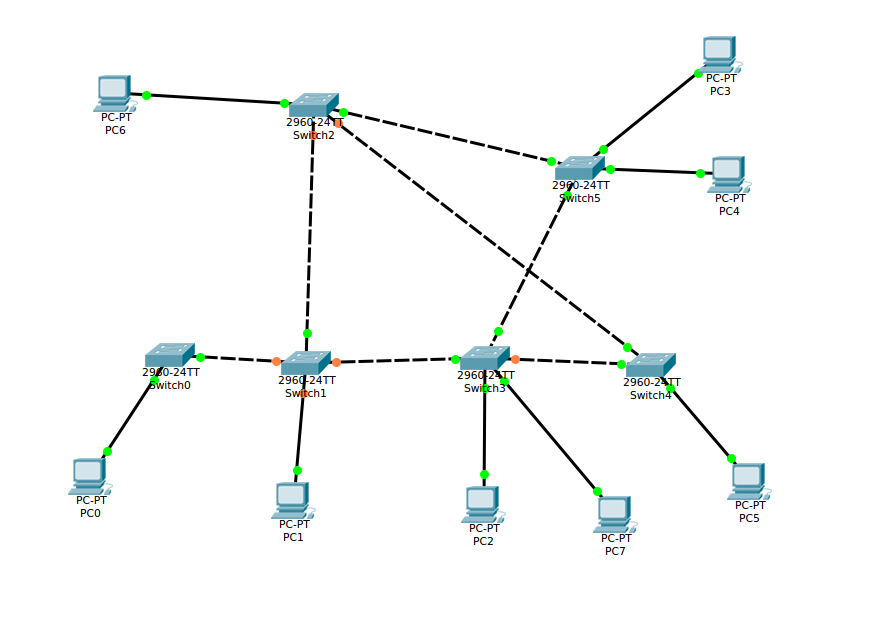
\includegraphics[scale=.6]{imagenes/A4e.png}
	\linebreak
\end{figure}

\subsection{¿Cuál es la diferencia del modo Access y el modo Trunk en un switch?}
La diferencia se encuentra que en el modo Access permite el paso de una VLAN, mientras que el modo Trunk permite el paso de un conjunto de VLAN

\subsection{¿Qué ocurre si conecto una puerta en modo Trunk a un PC?}
Este PC pasaría a formar parte de todas las VLAN conectadas a el por medio de la puerta en modo trunk.

\subsection{¿Qué ocurre si conecto dos switches, uno en modo access y otro en modo trunk?}
Entre ellos funcionarían como si ambos switches estuvieran en modo access con la VLAN del switch en modo access pues cualquier paquete de otra VLAN enviado por el switch en modo trunk seria descartado y este tampoco recibiría paquetes de esas VLAN porque el otro switch no los enviaría.

\subsection{¿Qué camino realizara un paquete que para llegar desde el switch 1 hasta el switch 0?}

Seguirá el camino de el enlace que comparten.

\chapter{Conclusión}
Los resultados de las actividades relacionadas al STP nos mostraron que éste bloquea puertos de forma automática para evitar bucles, también notamos que la prioridad y la asignación de switch primario y secundarios afectan el criterio con el que el protocolo elige que puertos bloquear. En la actividad de VLAN  vimos que la asignación de diferentes VLAN impide que interactúen equipos que no formen parte de la misma VLAN por medio de los switch que filtran el paso de los paquetes, de esto se concluye que este método hace que cada VLAN funcione como una red independiente sin que lo sean físicamente.

\listoffigures


\end{document}